%Correct the file name.
%X: book number
%Y: part number
%ZZZ: page number in three digits. So page 3 would be 003.

\documentclass[11pt]{amsbook}

\usepackage{../HBSuerDemir}	% ------------------------
\usepackage{enumerate}% http://ctan.org/pkg/enumerate
\usepackage{enumitem}
\usepackage{amsmath,amssymb}
\usepackage{amsfonts}

\begin{document}

% ++++++++++++++++++++++++++++++++++++++
\hPage{b2p2/405}
% ++++++++++++++++++++++++++++++++++++++



\begin{enumerate}[{1.}]	
	\item 
	Sketch the region of integration, and evaluate:
	
	$$
		a) \int_{-1} ^ {2} \int_{x^2} ^ {x+2}  \,dy \, dx         \qquad
		b)  \int_{0} ^ {\pi} \int_{0} ^ {1- \cos(\theta)}  \,dr \, d\theta  
	$$	
	
	\item
	Same question for:
	
	$$
		a ) 
		  \int_{0} ^ {a} \int_{a-x} ^ {\sqrt{a^2 - x^2}} \,y \,dy \, dx   \qquad	
		b ) 
		 \int_{0} ^ {a} \int_{- \sqrt{a^2 - x^2}} ^ {\sqrt{a^2 - x^2}}  \,dy \, dx  
	$$
	
	\item
	Sketch the region of integration and compute	
	
	$$ \int_{0} ^ {\frac{\pi}{2}} \int_{0} ^ {3 \sec(\theta -\frac{\pi}{6} )}  
	\,r \,dr \, d\theta  $$. 
	
	\item
	Without evaluating, find the largest and smallest possible
	value of
	
	$$
	\int  \int_{R}  \, {\sqrt{1 + x^2 + y^2}}  \,dA  
	$$
	where R is the region bounded by the curves
	$ y = 3x - x^2 $ and
	$ y = x^2 - 3x $ (Property 6).
	
	\item
	Same question for:
	
	$$
	a ) 
	\int_{-3} ^ {2} \int_{0} ^ {x+3} \,xy \,dy \, dx   \qquad	
	b ) 
	\int_{-2} ^ {3} \int_{-2} ^ {x+2}  \left( x^2 + y^2 \right) \,dy \, dx  
	$$
	
	\item
	Determine  $ a > 0$ such that
	
		$$
		\int  \int_{R} \left( x^2 + y^2\right)   \,dy \, dx =
		\int  \int_{R} \left( x^2 + y^2\right)   \,dx \, dy 
		$$
		
		\begin{figure}[htb]
	    \centering
	    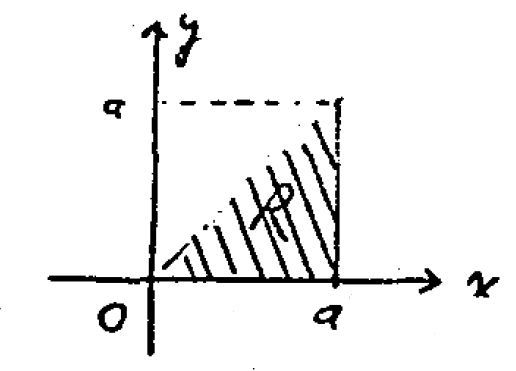
\includegraphics[width=0.3\textwidth]{images/b2p2_page405_figure_001}
        \end{figure}
		
	\item
	Evaluate
			$$
			\int  \int_{R_{\theta r } } \,xy   \,dA  
			$$
		where $ R_{ \theta r  } $
		is the polar region bounded 
		by  two circles shown in the Fig.
		
	    \begin{figure}[htb]
	        \centering
	        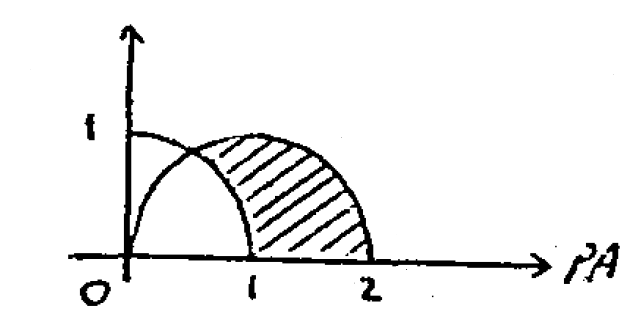
\includegraphics[width=0.3\textwidth]{images/b2p2_page405_figure_002}
        \end{figure}
	
	\item
	Evaluate
	$$
	\int  \int_{R}   \frac{dA}{ (x+y)^3 } 
	$$
	
	$$ \text{where } R =\left\lbrace 
	 \left( x,y \right) :  
	  x\geq1 ,
	  y\geq1,
	  x+y<3
	\right\rbrace  $$.
	
	\item
	Given
	
	\end{enumerate}	



% =======================================================
\end{document}  
